\documentclass[
  a4paper,
  oneside,
  BCOR = 10mm,
  DIV = 12,
  12pt,
  headings = normal,
]{scrartcl}

%%% Length calculations
\usepackage{calc}
%%%

%%% Support for color
\usepackage{xcolor}
\definecolor{lightblue}{HTML}{03A9F4}
\definecolor{red}{HTML}{F44336}
%%%

%%% Including graphics
\usepackage{graphicx}
%%%

%%% Font selection
\usepackage{fontspec}

\setromanfont{STIX Two Text}[
  SmallCapsFeatures = {LetterSpace = 8},
]

\setsansfont{IBM Plex Sans}[
  Scale = MatchUppercase,
]

\setmonofont{IBM Plex Mono}[
  Scale = MatchUppercase,
]
%%%

%%% Math typesetting
\usepackage{amsmath}

\usepackage{unicode-math}
\setmathfont{STIX Two Math}

\usepackage{IEEEtrantools}
%%%

%%% List settings
\usepackage{enumitem}
\setlist[enumerate]{
  label*      = {\arabic*.},
  left        = \parindent,
  topsep      = 0\baselineskip,
  parsep      = 0\baselineskip,
  noitemsep, % override itemsep
}
% List settings for levels 2–4
\setlist[enumerate, 2, 3, 4]{
  label*      = {\arabic*.},
  left        = 0em,
  topsep      = 0\baselineskip,
  parsep      = 0\baselineskip,
  noitemsep, % override itemsep
}

\setlist[itemize]{
  label*      = {—},
  left        = \parindent,
  topsep      = 0\baselineskip,
  parsep      = 0\baselineskip,
  itemsep     = 1\baselineskip,
  noitemsep, % override itemsep
}

\setlist[description]{
  font        = {\rmfamily\upshape\bfseries},
  topsep      = 1\baselineskip,
  parsep      = 0\baselineskip,
  itemsep     = 0\baselineskip,
}

%%%

%%% Structural elements typesetting
\setkomafont{pagenumber}{\rmfamily\upshape}
\setkomafont{disposition}{\rmfamily\bfseries}

% Sectioning
\RedeclareSectionCommand[
  beforeskip = -1\baselineskip,
  afterskip  = 1\baselineskip,
  font       = {\normalsize\bfseries\scshape},
]{section}

\RedeclareSectionCommand[
  beforeskip = -1\baselineskip,
  afterskip  = 1\baselineskip,
  font       = {\normalsize\bfseries\itshape},
]{subsection}

\RedeclareSectionCommand[
  beforeskip = -1\baselineskip,
  afterskip  = 1\baselineskip,
  font       = {\normalsize\bfseries},
]{subsubsection}

\RedeclareSectionCommand[
  beforeskip = -1\baselineskip,
  afterskip  = -0.5em,
  font       = {\normalsize\mdseries\scshape\addfontfeatures{Letters = {UppercaseSmallCaps}}},
]{paragraph}
%%%

%%% Typographic enhancements
\usepackage{microtype}
%%%

%%% Language-specific settings
\usepackage{polyglossia}
\setmainlanguage{ukrainian}
\setotherlanguages{english}
%%%

%%% Captions
\usepackage{caption}
\usepackage{subcaption}

%\DeclareCaptionLabelFormat{closing}{#2)}
%\captionsetup[subtable]{labelformat = closing}

%\captionsetup[subfigure]{labelformat = closing}

\captionsetup[table]{
  aboveskip = 0\baselineskip,
  belowskip = 0\baselineskip,
}

\captionsetup[figure]{
  aboveskip = 1\baselineskip,
  belowskip = 0\baselineskip,
}

\captionsetup[subfigure]{
  labelformat = simple,
  labelformat = brace,
  justification = RaggedRight,
  singlelinecheck = false,
}
%%%

%%% Hyphenated ragged typesetting
\usepackage{ragged2e}
%%%

%%% Table typesetting
\usepackage{booktabs}
\usepackage{longtable}

\usepackage{multirow}

\usepackage{array}
\newcolumntype{v}[1]{>{\RaggedRight\arraybackslash\hspace{0pt}}p{#1}}
\newcolumntype{b}[1]{>{\Centering\arraybackslash\hspace{0pt}}p{#1}}
\newcolumntype{n}[1]{>{\RaggedLeft\arraybackslash\hspace{0pt}}p{#1}}
%%%

%%% Drawing
\usepackage{tikz}
\usepackage{tikzscale}
\usetikzlibrary{arrows.meta} % Stealth arrow tips
\usetikzlibrary{backgrounds} % Stealth arrow tips
\usetikzlibrary{datavisualization.formats.functions}
\usetikzlibrary{datavisualization}
\usetikzlibrary{fit}
\usetikzlibrary{graphdrawing}
\usegdlibrary{trees}
\usetikzlibrary{graphs}
\usetikzlibrary{intersections}
\usetikzlibrary{patterns}
\usetikzlibrary{positioning}
\usetikzlibrary{shapes.geometric}
\usetikzlibrary{quotes}

\usepackage{pgfplots}
\usepgfplotslibrary{fillbetween}
%%%

%%% SI units typesetting
\usepackage{siunitx}
\sisetup{
  output-decimal-marker = {,},
  exponent-product      = {\cdot},
  inter-unit-product    = \ensuremath{{} \cdot {}},
  per-mode              = symbol,
}
%%%

% Code Highlighting
\usepackage{minted}
\setmintedinline{
  style = bw,
  breaklines,
}

\newminted[bashterm]{text}{%
  autogobble,%
  breaklines,%
  style=bw,%
}

\newminted[codegeneric]{text}{%
  autogobble,%
  style=bw,%
  breaklines,%
  fontsize=\small,%
}

\newmintinline{bash}{%
}

\newmintinline[minttext]{text}{%
  breaklines,%
  breakanywhere,%
}

%%% Framing code listings
\usepackage{tcolorbox}
\tcbuselibrary{breakable}
\tcbuselibrary{minted}
\tcbuselibrary{skins}

% Text file listing
\newtcblisting[
  auto counter,
  list inside,
  number within = section,
]{listingplaintext}[3][]{%
  minted language = text,
  minted style    = bw,
  minted options  = {
    autogobble,
    linenos,
    tabsize = 4,
    breaklines,
    breakanywhere,
    fontsize = \footnotesize,
  },
  empty,
  sharp corners,
  coltitle = black,
  borderline horizontal = {1pt}{0pt}{black},
  titlerule = {0.5pt},
  titlerule style = {
    black,
  },
  toptitle = 0.3em,
  bottomtitle = 0.3em,
  before skip      = \intextsep,
  after  skip      = \intextsep,
  title            = {Лістинг \thetcbcounter: #2},
  list entry       = {\protect\numberline{\thetcbcounter}#2},
  left = 0em,
  right = 0em,
  %
  listing only,
  breakable,
  %
  label = {#3},%
}

\newtcbinputlisting[
  use counter from = listingplaintext,
  list inside,
  number within = section
]{\inputplaintext}[4][]{%
  minted language = text,
  minted style    = bw,
  minted options  = {
    autogobble,
    linenos,
    tabsize = 4,
    breaklines,
    breakanywhere,
    fontsize = \footnotesize,
  },
  empty,
  sharp corners,
  coltitle = black,
  borderline horizontal = {1pt}{0pt}{black},
  titlerule = {0.5pt},
  titlerule style = {
    black,
  },
  toptitle = 0.3em,
  bottomtitle = 0.3em,
  before skip      = \intextsep,
  after  skip      = \intextsep,
  title            = {Лістинг \thetcbcounter: #3},
  list entry       = {\protect\numberline{\thetcbcounter}#3},
  left = 0em,
  right = 0em,
  %
  listing file={#2},
  listing only,
  breakable,
  %
  label = {#4}
}

\newtcblisting[
  use counter from = listingplaintext,
  list inside,
  number within = section,
]{listingpython}[3][]{%
  minted language = python,
  minted style    = bw,
  minted options  = {
    autogobble,
    linenos,
    tabsize = 4,
    breaklines,
    breakanywhere,
    fontsize = \footnotesize,
  },
  empty,
  sharp corners,
  coltitle = black,
  borderline horizontal = {1pt}{0pt}{black},
  titlerule = {0.5pt},
  titlerule style = {
    black,
  },
  toptitle = 0.3em,
  bottomtitle = 0.3em,
  before skip      = \intextsep,
  after  skip      = \intextsep,
  title            = {Лістинг \thetcbcounter: #2},
  list entry       = {\protect\numberline{\thetcbcounter}#2},
  left = 0em,
  right = 0em,
  %
  listing only,
  breakable,
  %
  label = {#3},
  %
  #1%
}

\newtcbinputlisting[
  use counter from = listingplaintext,
  list inside,
  number within = section
]{\inputpython}[4][]{%
  minted language = python,
  minted style    = bw,
  minted options  = {
    autogobble,
    linenos,
    tabsize = 4,
    breaklines,
    breakanywhere,
    fontsize = \footnotesize,
  },
  empty,
  sharp corners,
  coltitle = black,
  borderline horizontal = {1pt}{0pt}{black},
  titlerule = {0.5pt},
  titlerule style = {
    black,
  },
  toptitle = 0.3em,
  bottomtitle = 0.3em,
  before skip      = \intextsep,
  after  skip      = \intextsep,
  title            = {Лістинг \thetcbcounter: #3},
  list entry       = {\protect\numberline{\thetcbcounter}#3},
  left = 0em,
  right = 0em,
  %
  listing file={#2},
  listing only,
  breakable,
  %
  label = {#4}
}

\newtcbinputlisting[
  use counter from = listingplaintext,
  list inside,
  number within = section
]{\inputada}[4][]{%
  minted language = ada,
  minted style    = bw,
  minted options  = {
    autogobble,
    linenos,
    tabsize = 4,
    breaklines,
    breakanywhere,
    fontsize = \footnotesize,
  },
  empty,
  sharp corners,
  coltitle = black,
  borderline horizontal = {1pt}{0pt}{black},
  titlerule = {0.5pt},
  titlerule style = {
    black,
  },
  toptitle = 0.3em,
  bottomtitle = 0.3em,
  before skip      = \intextsep,
  after  skip      = \intextsep,
  title            = {Лістинг \thetcbcounter: #3},
  list entry       = {\protect\numberline{\thetcbcounter}#3},
  left = 0em,
  right = 0em,
  %
  listing file={#2},
  listing only,
  breakable,
  %
  label = {#4}
}

% Linux command-line listing
\newtcblisting{linuxterm}%
{%
  % Syntax highlighing options
  listing only,%
  minted language = bash,%
  minted options={%
    autogobble,%
    linenos%
  },%
  % Presentation options
  empty,%
  %% Margins
  sharp corners,%
  toptitle = 0.0em,%
  bottomtitle = 0.0em,%
  left = 0em,%
  right = 0em,%
  before skip = \intextsep,%
  after skip = \intextsep,%
}

\newtcblisting{linuxtermout}%
{%
  % Syntax highlighing options
  listing only,%
  minted language = text,%
  minted options={%
    autogobble,%
    linenos%
  },%
  % Presentation options
  empty,%
  %% Margins
  sharp corners,%
  toptitle = 0.0em,%
  bottomtitle = 0.0em,%
  left = 0em,%
  right = 0em,%
  before skip = \intextsep,%
  after skip = \intextsep,%
}

% Dockerfile listings
\newtcblisting[
  use counter from = listingplaintext,
  list inside,
  number within = section,
]{listingdocker}[3][]{%
  minted language = dockerfile,
  minted style    = bw,
  minted options  = {
    autogobble,%
    linenos,
    tabsize = 4,
    breaklines,
    breakanywhere,
    fontsize = \footnotesize,
  },
  empty,
  sharp corners,
  coltitle = black,
  borderline horizontal = {1pt}{0pt}{black},
  titlerule = {0.5pt},
  titlerule style = {
    black,
  },
  toptitle = 0.3em,
  bottomtitle = 0.3em,
  before skip      = \intextsep,
  after  skip      = \intextsep,
  title            = {Лістинг \thetcbcounter: #2},
  list entry       = {\protect\numberline{\thetcbcounter}#2},
  left = 0em,
  right = 0em,
  %
  listing only,
  breakable,
  %
  label = {#3},%
}

% Docker Compose listings
\newtcblisting[
  use counter from = listingplaintext,
  list inside,
  number within = section,
]{listingdockercompose}[3][]{%
  minted language = yaml,
  minted style    = bw,
  minted options  = {
    autogobble,%
    linenos,
    tabsize = 4,
    breaklines,
    breakanywhere,
    fontsize = \footnotesize,
  },
  empty,
  sharp corners,
  coltitle = black,
  borderline horizontal = {1pt}{0pt}{black},
  titlerule = {0.5pt},
  titlerule style = {
    black,
  },
  toptitle = 0.3em,
  bottomtitle = 0.3em,
  before skip      = \intextsep,
  after  skip      = \intextsep,
  title            = {Лістинг \thetcbcounter: #2},
  list entry       = {\protect\numberline{\thetcbcounter}#2},
  left = 0em,
  right = 0em,
  %
  listing only,
  breakable,
  %
  label = {#3},%
}


% Customize minted line numbers
\renewcommand{\theFancyVerbLine}{\ttfamily\scriptsize\arabic{FancyVerbLine}}

%%%

%%% Typeset menus and keys
\usepackage{menukeys}[
  os=win,
]
%%%

%%% Links and hyperreferences
\usepackage{hyperref}
\hypersetup{
  bookmarksnumbered = true,
  colorlinks      = false,
  linkbordercolor = red,
  urlbordercolor  = lightblue,
  pdfborderstyle  = {/S/U/W 1.5},
}
%%%

%%% Length adjustment

% Set baselineskip, default is 14.5 pt
\linespread{1.068966} % ~15.5 pt
\setlength{\emergencystretch}{1em}
\setlength{\parindent}{1.5em}
\newlength{\gridunitwidth}
\setlength{\gridunitwidth}{\textwidth / 12}
%%%

%%% Custom commands
\newcommand{\allcaps}[1]{%
  {%
    \addfontfeatures{%
      Letters = UppercaseSmallCaps,
      LetterSpace = 8,%
    }%
    #1%
  }%
}
\newcommand{\filename}[1]{\texttt{#1}}
\newcommand{\progname}[1]{\texttt{#1}}
\newcommand{\commandname}[1]{\texttt{#1}}
\newcommand{\modulename}[1]{\texttt{#1}}
\newcommand{\transeng}[1]{{англ.}~\textit{\textenglish{#1}}}
%%%

%%% Custom math commands
\newcommand{\longvar}[1]{\mathit{#1}}
\newcommand{\vect}[1]{\mathbfit{#1}}
\newcommand{\matr}[1]{\mathbfit{#1}}

\newcommand{\logequiv}{\mathrel{\Longleftrightarrow}} % Logically equivalent

\DeclareMathOperator*{\minimize}{min} % minimize for linear programs
%%%

%%% Custom drawing commands
\makeatletter
\newcommand{\Distance}[3]{% % from https://tex.stackexchange.com/q/56353/121799
\tikz@scan@one@point\pgfutil@firstofone($#1-#2$)\relax  
\pgfmathsetmacro{#3}{veclen(\the\pgf@x,\the\pgf@y)}
}% Explanation: the calc library allows us, among other things, to add and
% subtract points, so ($#1-#2$) is simply the difference between the points
% #1 and #2. The combination \tikz@scan@one@point\pgfutil@firstofone extracts
% the coordinates of the new point and stores them in \pgf@x and \pgf@y.
% They get fed in veclen, and \pgfmathsetmacro stores the result in #3.
% EDIT: included fudge factor, see https://tex.stackexchange.com/a/22702/121799
\makeatother
%%%

\begin{document}

\begin{titlepage}
    \begin{center}
      Міністерство освіти і~науки України\\
      Національний авіаційний університет\\
      Факультет кібербезпеки, комп'ютерної та~програмної інженерії\\
      Кафедра комп'ютеризованих систем управління

      \vspace{\fill}
        Лабораторна робота №~1.1\\
        з~дисципліни «Паралельні і~розподілені обчислення»\\
        на~тему «Ада. Семафори»

      \vspace{\fill}

      \begin{flushright}
        Виконав:\\
        студент \allcaps{ФККПІ}\\
        групи \allcaps{СП}-425\\
        Клокун В.\,Д.\\
        Перевірив:\\
        Корочкін О.\,В.
      \end{flushright}

      Київ 2019
    \end{center}
  \end{titlepage}

  \section{Завдання роботи}
    Розробити програму для~заданої паралельної комп'ютерної системи зі~спільною пам'яттю~(рис.~\ref{fig:task-sys}).

    \begin{figure}[!htbp]
      \centering
      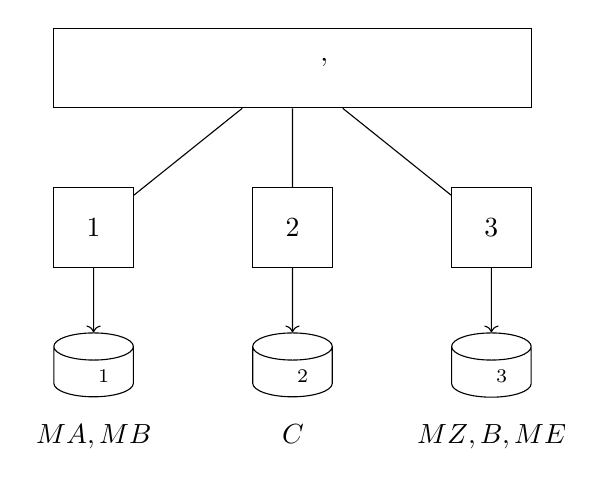
\begin{tikzpicture}[
        iod/.style = {
          draw,
          cylinder,
          shape border rotate = 90,
          minimum width = \gridunitwidth,
          aspect = 0.5,
        },
        memd/.style = {
          draw,
          rectangle,
          minimum height = 1\gridunitwidth,
          minimum width = 6\gridunitwidth,
        },
        thread/.style = {
          draw,
          rectangle,
          minimum width = \gridunitwidth,
          minimum height = \gridunitwidth,
        }
      ]
        \node (mem) at (0,0) [
          memd,
        ] {Спільна пам'ять};

        \node (t1) [
          thread,
          below = of mem.south west,
          anchor = north west,
        ] {1};

        \node (iod1) [
          iod,
          below = of t1.south west,
          anchor = before top,
        ] {$\text{ПВВ}_{1}$};

        \node (vars1) [
          below = 0.5 \baselineskip of iod1,
        ] {$MA, MB$};

        \node (t2) [
          thread,
          below = of mem.south,
          anchor = north,
        ] {2};

        \node (iod2) [
          iod,
          below = of t2.south west,
          anchor = before top,
        ] {$\text{ПВВ}_{2}$};

        \node (vars2) [
          below = 0.5 \baselineskip of iod2,
        ] {$C$};

        \node (t3) [
          thread,
          below = of mem.south east,
          anchor = north east,
        ] {3};

        \node (iod3) [
          iod,
          below = of t3.south west,
          anchor = before top,
        ] {$\text{ПВВ}_{3}$};

        \node (vars3) [
          below = 0.5 \baselineskip of iod3,
        ] {$MZ, B, ME$};

        \draw [->] (mem) -- (t1) -- (iod1);
        \draw [->] (mem) -- (t2) -- (iod2);
        \draw [->] (mem) -- (t3) -- (iod3);
      \end{tikzpicture}
      \caption{Задана паралельна комп'ютерна система зі~спільною пам'яттю}
      \label{fig:task-sys}
    \end{figure}

    Програма, розроблена для~даної системи, повинна обчислювати значення такого виразу:
    \begin{IEEEeqnarray*}{rCl}
      MA = ( MB \cdot MZ ) + (B \cdot C) \cdot ME.
    \end{IEEEeqnarray*}
    Розробити програму на~мові програмування «Ада», використовуючи для~взаємодії потоків (задач) семафори мови «Ада» з~пакету \minttext{Ada.Synchronous_Task_Control}.

  \section{Хід~роботи}
    \subsection{Побудова паралельного алгоритму}
      Необхідно паралельно обчислити значення виразу $MA = ( MB \cdot MZ ) + (B \cdot C) \cdot ME$. Для~цього складаємо паралельний алгоритм:
      \begin{enumerate}
        \item Позначимо скалярний добуток векторів як~$a = B \cdot C$.
        \item Обчислимо частини, які~складатимуть скалярний добуток векторів:
          \begin{IEEEeqnarray*}{rCl}
            a = B_{H_{1}} \cdot C_{H_{1}}, \quad
            a_{i} = B_{H_{i}} \cdot C_{H_{i}}, \quad
            a \in \{2, 3\}.
          \end{IEEEeqnarray*}
        \item Обчислимо скалярний добуток векторів, склавши частини:
          \begin{IEEEeqnarray*}{rCl}
            a = a + a_{2} + a_{3}.
          \end{IEEEeqnarray*}
        \item Паралельно обчислюємо матрицю-результат по~частинам:
          \begin{IEEEeqnarray*}{rCl}
            MA_{H_{i}} = (MB_{H_{i}} \cdot MZ) + a \cdot ME_{H_{i}}, \quad
            a \in \{1, 2, 3\}.
          \end{IEEEeqnarray*}
      \end{enumerate}
      Спільні ресурси: $a, a_{2}, a_{3}$~— для~обчислення скалярного добутку; $MZ$~— для~множення матриць.

    \subsection{Розробка алгоритмів потоків (задач)}
      Розробивши паралельний алгоритм, переходимо до~розробки алгоритмів потоків. Представимо їх~у~вигляді таблиці.

      \begin{longtable}{
        v{8\gridunitwidth - 2\tabcolsep}
        n{4\gridunitwidth - 2\tabcolsep}
      }
          \caption{Паралельний алгоритм потоку 1}\label{fig:task1-alg}\\
          \toprule
            Дія~& Точки синхронізації\\
          \midrule
        \endfirsthead
          \caption{Паралельний алгоритм потоку 1}\\
          \toprule
            Дія~& Точки синхронізації\\
          \midrule
        \endhead
          \bottomrule
        \endfoot
        %
          Ввести $MB$\\
          Подати сигнал, що~$MB$ введена, в~задачу $T2$ & $S_{2,MB}$\\
          Подати сигнал, що~$MB$ введена, в~задачу $T3$ & $S_{3,MB}$\\
          Очікувати введення~$C$ & $W_{1,C}$\\
          Очікувати введення~$MZ, B, ME$ & $W_{1,MZBME}$\\
          Скопіювати $MZ_{1} \coloneq MZ$ & Критична ділянка\\
          Обчислити $a \coloneq C_{H_{1}} \cdot B_{H_{1}}$ & Критична ділянка\\
          Чекати готовності $a_2$ із~задачі $T2$ & $W_{1,a_{2}}$\\
          Чекати готовності $a_3$ із~задачі $T3$ & $W_{1,a_{3}}$\\
          Обчислити $a = a + a_{2} + a_{3}$ & Критична ділянка\\
          Подати сигнал, що~готове значення~$a$, в~задачу~$T2$ & $S_{2,a}$\\
          Подати сигнал, що~готове значення~$a$, в~задачу~$T3$ & $S_{3,a}$\\
          Обчислити $MA_{H_{1}} = (MB_{H_{1}} \cdot MZ_{1}) + a \cdot ME_{H_{1}}$\\
          Очікувати готовності $MA_{H_{2}}$ від~задачі $T2$ & $W_{1, MA_{H_{2}}}$\\
          Очікувати готовності $MA_{H_{3}}$ від~задачі $T3$ & $W_{1, MA_{H_{3}}}$\\
          Вивести $MA$
      \end{longtable}

      \begin{longtable}{
        v{8\gridunitwidth - 2\tabcolsep}
        n{4\gridunitwidth - 2\tabcolsep}
      }
          \caption{Паралельний алгоритм потоку 2}\label{fig:task2-alg}\\
          \toprule
            Дія~& Точки синхронізації\\
          \midrule
        \endfirsthead
          \caption{Паралельний алгоритм потоку 2}\\
          \toprule
            Дія~& Точки синхронізації\\
          \midrule
        \endhead
          \bottomrule
        \endfoot
        %
          Ввести $C$\\
          Подати сигнал, що~$C$ введена, в~задачу $T1$ & $S_{1,C}$\\
          Подати сигнал, що~$C$ введена, в~задачу $T3$ & $S_{3,C}$\\
          Очікувати введення~$MZ, B, ME$ & $W_{2,MZBME}$\\
          Скопіювати $MZ_{2} \coloneq MZ$ & Критична ділянка\\
          Обчислити $a_{2} \coloneq C_{H_{2}} \cdot B_{H_{2}}$ & Критична ділянка\\
          Подати сигнал, що~готове значення~$a_2$, в~задачу~$T1$ & $S_{1,a_{2}}$\\
          Очікувати готовності $a$ від~задачі $T1$ & $W_{2,a}$\\
          Скопіювати значення $ac_2 \coloneq a$ & Критична ділянка\\
          Очікувати введення~$MB$ & $W_{2,MB}$\\
          Обчислити $MA_{H_{2}} = (MB_{H_{2}} \cdot MZ_{H_{2}}) + a \cdot ME_{H_{2}}$\\
          Дати сигнал, що~готове значення $MA_{H_{2}}$, задачі $T1$ & $S_{1, MA_{H_{2}}}$
      \end{longtable}

      \begin{longtable}{
        v{8\gridunitwidth - 2\tabcolsep}
        n{4\gridunitwidth - 2\tabcolsep}
      }
          \caption{Паралельний алгоритм потоку 3}\label{fig:task3-alg}\\
          \toprule
            Дія~& Точки синхронізації\\
          \midrule
        \endfirsthead
          \caption{Паралельний алгоритм потоку 3}\\
          \toprule
            Дія~& Точки синхронізації\\
          \midrule
        \endhead
          \bottomrule
        \endfoot
        %
          Ввести $MZ, B, ME$\\
          Подати сигнал, що~$MZ, B, ME$ введені, в~задачу $T1$ & $S_{1,MZBME}$\\
          Подати сигнал, що~$MZ, B, ME$ введені, в~задачу $T2$ & $S_{2,MZBME}$\\
          Очікувати введення~$C$ & $W_{3,C}$\\
          Обчислити $a_{3} \coloneq C_{H_{3}} \cdot B_{H_{3}}$ & Критична ділянка\\
          Подати сигнал, що~готове значення~$a_3$, в~задачу~$T1$ & $S_{1,a_{3}}$\\
          Очікувати готовності $a$ від~задачі $T1$ & $W_{3,a}$\\
          Скопіювати значення $ac_3 \coloneq a$ & Критична ділянка\\
          Очікувати введення~$MB$ & $W_{3,MB}$\\
          Обчислити $MA_{H_{3}} = (MB_{H_{3}} \cdot MZ_{H_{3}}) + a \cdot ME_{H_{3}}$\\
          Дати сигнал, що~готове значення $MA_{H_{3}}$, задачі $T1$ & $S_{1, MA_{H_{3}}}$
      \end{longtable}

    \subsection{Розробка структурної схеми взаємодії задач}
      Розроблюємо структурну схему взаємодії задач~(рис.~\ref{fig:struct-interaction}). Розробивши схему, вкажемо, навіщо призначені семафори, які~в~ній~використовуються:
      \begin{description}[
        leftmargin = 2.5\gridunitwidth,
        style = nextline,
      ]
        \item [$\text{Sem}_{cr}$] Призначений для~доступу до~спільних ресурсів.
        \item [$\text{Sem}_{2,MB}$] Призначений для~синхронізації задачі~$T2$ після введення~$MB$.
        \item [$\text{Sem}_{3,MB}$] Призначений для~синхронізації задачі~$T3$ після введення~$MB$.
        \item [$\text{Sem}_{2,a}$] Призначений для~синхронізації задачі~$T2$ після обчислення~$a$.
        \item [$\text{Sem}_{3,a}$] Призначений для~синхронізації задачі~$T3$ після обчислення~$a$.
        \item [$\text{Sem}_{1,C}$] Призначений для~синхронізації задачі~$T1$ після введення~$C$.
        \item [$\text{Sem}_{3,C}$] Призначений для~синхронізації задачі~$T3$ після введення~$C$.
        \item [$\text{Sem}_{1,a_{2}}$] Призначений для~синхронізації задачі~$T1$ після обчислення~$a_2$.
        \item [$\text{Sem}_{1,MA_{H_{2}}}$] Призначений для~синхронізації задачі~$T1$ після обчислення~$MA_{H_{2}}$.
        \item [$\text{Sem}_{1,MZBME}$] Призначений для~синхронізації задачі~$T1$ після введення~$MZ$, $B$, $ME$.
        \item [$\text{Sem}_{2,MZBME}$] Призначений для~синхронізації задачі~$T2$ після введення~$MZ$, $B$, $ME$.
        \item [$\text{Sem}_{1,a_{3}}$] Призначений для~синхронізації задачі~$T1$ після обчислення~$a_3$.
        \item [$\text{Sem}_{1,MA_{H_{3}}}$] Призначений для~синхронізації задачі~$T3$ після обчислення~$MA_{H_{2}}$.
      \end{description}
      Після розробки структурної схеми можна переходити до~розробки програми.

      \begin{figure}[!htbp]
        \centering
        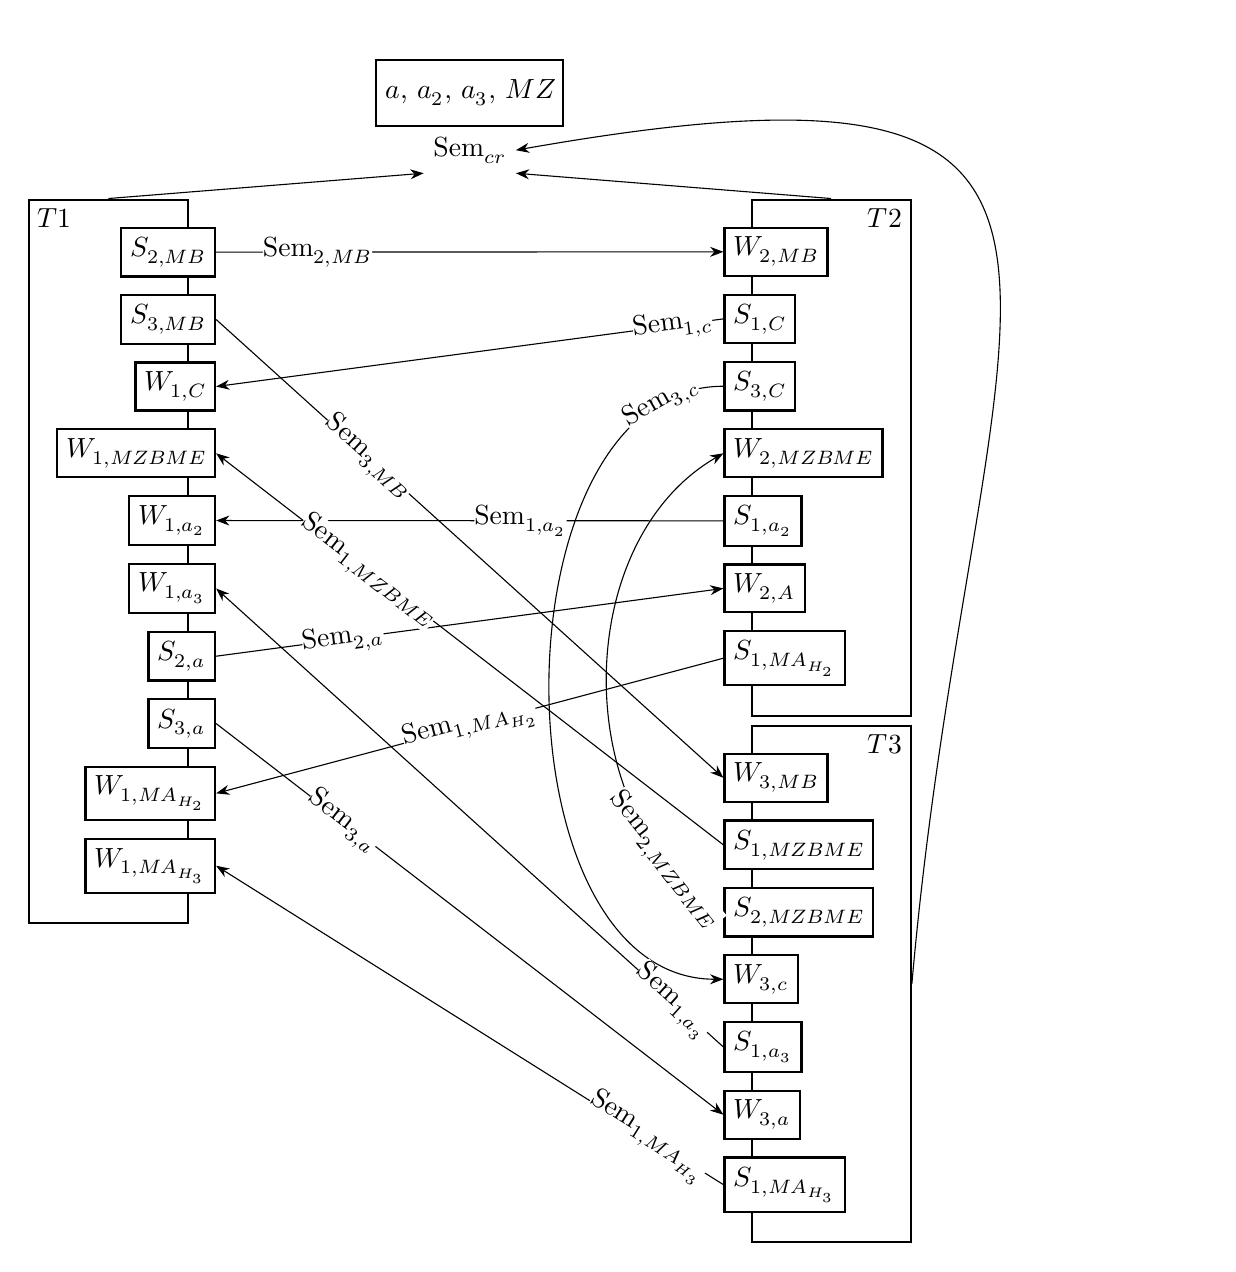
\begin{tikzpicture}[
            resource/.style = {
              draw,
              thick,
            },
            thread/.style = {
              draw,
              rectangle,
              thick,
            },
            syncobj/.style = {
              draw,
              rectangle,
              fill = white,
              thick,
            },
        ]
          \begin{scope}
            \node (x) at (0,0) [
              resource,
              minimum height = 2 \baselineskip,
              minimum width = 2 \baselineskip,
              label = {
                []above:Спільний ресурс
              },
              label = {
                [name = xlabel node]below:$\text{Sem}_{cr}$
              },
            ] {$a$, $a_2$, $a_3$, $MZ$};
          \end{scope}

          % Thread 1
          \begin{scope}[
            syncobj/.append style = {
            },
          ]
            \node (s2mb) [
              syncobj,
              below = 3 \baselineskip of x.south west,
              xshift = -2\gridunitwidth,
              anchor = north east,
            ] {$S_{2, MB}$};

            \node (s3mb) [
              syncobj,
              below = 0.5 \baselineskip of s2mb.south east,
              anchor = north east,
            ] {$S_{3, MB}$};

            \node (w1c) [
              syncobj,
              below = 0.5 \baselineskip of s3mb.south east,
              anchor = north east,
            ]
            {$W_{1, C}$};

            \node (w1mzbme) [
              syncobj,
              below = 0.5 \baselineskip of w1c.south east,
              anchor = north east,
            ] {$W_{1, MZBME}$};

            \node (w1a2) [
              syncobj,
              below = 0.5 \baselineskip of w1mzbme.south east,
              anchor = north east,
            ] {$W_{1, a_{2}}$};

            \node (w1a3) [
              syncobj,
              below = 0.5 \baselineskip of w1a2.south east,
              anchor = north east,
            ] {$W_{1, a_{3}}$};

            \node (s2a) [
              syncobj,
              below = 0.5 \baselineskip of w1a3.south east,
              anchor = north east,
            ] {$S_{2, a}$};

            \node (s3a) [
              syncobj,
              below = 0.5 \baselineskip of s2a.south east,
              anchor = north east,
            ] {$S_{3, a}$};

            \node (w1mah2) [
              syncobj,
              below = 0.5 \baselineskip of s3a.south east,
              anchor = north east,
            ] {$W_{1, MA_{H_{2}}}$};

            \node (w1mah3) [
              syncobj,
              below = 0.5 \baselineskip of w1mah2.south east,
              anchor = north east,
            ] {$W_{1, MA_{H_{3}}}$};

            \begin{scope}[on background layer]
              \node [
                fit = {
                  (s2mb) (s3mb) (w1c) (w1mzbme) (w1a2) (w1a3) (s2a) (s3a)
                  (w1mah2) (w1mah3)
                },
                inner ysep = 1em,
                inner xsep = -1em,
              ] (t1fit)
              {};
              \Distance{(t1fit.north)}{(t1fit.south)}{\mylen}
              \node (t1) at (t1fit.north east) [
                anchor = north east,
                thread,
                minimum height = \mylen,
                minimum width = 2 \gridunitwidth,
                label={
                  [anchor = north west]north west:$T1$
                },
              ]
              {};
            \end{scope}
          \end{scope}

          % Thread 2
          \begin{scope}
            \node (w2mb) [
              syncobj,
              below = 3 \baselineskip of x.south east,
              xshift = 2 \gridunitwidth,
              anchor = north west,
            ]
            {$W_{2,MB}$};

            \node (s1c) [
              syncobj,
              below = 0.5\baselineskip of w2mb.south west,
              anchor = north west,
            ]
            {$S_{1,C}$};

            \node (s3c) [
              syncobj,
              below = 0.5\baselineskip of s1c.south west,
              anchor = north west,
            ]
            {$S_{3,C}$};

            \node (w2mzbme) [
              syncobj,
              below = 0.5\baselineskip of s3c.south west,
              anchor = north west,
            ]
            {$W_{2,MZBME}$};

            \node (s1a2) [
              syncobj,
              below = 0.5\baselineskip of w2mzbme.south west,
              anchor = north west,
            ]
            {$S_{1,a_{2}}$};

            \node (w2a) [
              syncobj,
              below = 0.5\baselineskip of s1a2.south west,
              anchor = north west,
            ]
            {$W_{2,A}$};

            \node (s1mah2) [
              syncobj,
              below = 0.5\baselineskip of w2a.south west,
              anchor = north west,
            ]
            {$S_{1,MA_{H_{2}}}$};

            \begin{scope}[on background layer]
              \node [
                fit = (w2mb) (s1c) (s3c) (w2mzbme) (s1a2) (w2a) (s1mah2),
                inner ysep = 1em,
                inner xsep = -1em,
              ] (t2fit)
              {};
              \Distance{(t2fit.north)}{(t2fit.south)}{\mylen}
              \node (t2) at (t2fit.north west) [
                anchor = north west,
                thread,
                minimum height = \mylen,
                minimum width = 2 \gridunitwidth,
                label={
                  [anchor = north east]north east:$T2$
                },
              ]
              {};
            \end{scope}
          \end{scope}

          \begin{scope}
            \node (w3mb) [
              syncobj,
              below = 2 \baselineskip of s1mah2.south west,
              anchor = north west,
            ]
            {$W_{3,MB}$};

            \node (s1mzbme) [
              syncobj,
              below = 0.5\baselineskip of w3mb.south west,
              anchor = north west,
            ]
            {$S_{1,MZBME}$};

            \node (s2mzbme) [
              syncobj,
              below = 0.5\baselineskip of s1mzbme.south west,
              anchor = north west,
            ]
            {$S_{2,MZBME}$};

            \node (w3c) [
              syncobj,
              below = 0.5\baselineskip of s2mzbme.south west,
              anchor = north west,
            ]
            {$W_{3,c}$};

            \node (s1a3) [
              syncobj,
              below = 0.5\baselineskip of w3c.south west,
              anchor = north west,
            ]
            {$S_{1,a_{3}}$};

            \node (w3a) [
              syncobj,
              below = 0.5\baselineskip of s1a3.south west,
              anchor = north west,
            ]
            {$W_{3,a}$};

            \node (s1mah3) [
              syncobj,
              below = 0.5\baselineskip of w3a.south west,
              anchor = north west,
            ]
            {$S_{1,MA_{H_{3}}}$};

            \begin{scope}[on background layer]
              \node [
                fit = (w3mb) (s1mzbme) (s2mzbme) (w3c) (s1a3) (w3a) (s1mah3),
                inner ysep = 1em,
                inner xsep = -1em,
              ] (t3fit)
              {};
              \Distance{(t3fit.north)}{(t3fit.south)}{\mylen}
              \node (t3) at (t3fit.north west) [
                anchor = north west,
                thread,
                minimum width = 2 \gridunitwidth,
                minimum height = \mylen,
                label = {
                  [anchor = north east]north east:$T3$
                },
              ]
              {};
            \end{scope}
          \end{scope}

          \begin{scope}[
            >=Stealth,
            elbl/.style = {
              fill = white,
              inner sep = 0em,
              pos = 0.1,
            },
            every edge/.append style = {
              sloped,
            }
          ]
            \path [->] (s2mb.east)
              edge
              node [elbl, pos=0.20] {$\text{Sem}_{2,MB}$}
              (w2mb.west);

            \path [->] (s3mb.east)
              edge
              node [elbl, pos=0.30] {$\text{Sem}_{3,MB}$}
              (w3mb.west);

            \path [->] (s2a.east)
              edge
              node [elbl, pos=0.25] {$\text{Sem}_{2,a}$}
              (w2a.west);

            \path [->] (s3a.east)
              edge
              node [elbl, pos=0.25] {$\text{Sem}_{3,a}$}
              (w3a.west);

            %
            \path [->] (s1c.west)
              edge
              node [elbl] {$\text{Sem}_{1,c}$}
              (w1c.east);

            \path [->] (s3c.west)
              edge
              [bend right = 90] node [elbl] {$\text{Sem}_{3,c}$}
              (w3c.west);

            \path [->] (s1a2.west)
              edge
              node [elbl, pos = 0.4] {$\text{Sem}_{1,a_{2}}$}
              (w1a2.east);

            \path [->] (s1mah2.west)
              edge
              node [elbl, pos = 0.5] {$\text{Sem}_{1,MA_{H_{2}}}$}
              (w1mah2.east);

            %
            \path [->] (s1mzbme.west)
              edge
              node [elbl, pos=0.7] {$\text{Sem}_{1,MZBME}$}
              (w1mzbme.east);
            \path [->] (s2mzbme.west)
              edge
              [bend left = 60]
              node [elbl, pos = 0.15] {$\text{Sem}_{2,MZBME}$}
              (w2mzbme.west);
            \path [->] (s1a3.west)
              edge
              node [elbl] {$\text{Sem}_{1,a_{3}}$}
              (w1a3.east);
            \path [->] (s1mah3.west)
              edge
              node [elbl, pos = 0.15] {$\text{Sem}_{1,MA_{H_{3}}}$}
              (w1mah3.east);

            % Shared resource node
            \path [->] (t1.north)
              edge
              node [] {}
              (xlabel node.south west);

            \path [->] (t2.north)
              edge
              node [] {}
              (xlabel node.south east);

            \path [->] (t3.east)
              edge [out=85, in=10, looseness=1.95]
              node [] {}
              (xlabel node.east);
          \end{scope}
        \end{tikzpicture}
        \caption{Структурна схема взаємодії задач}
        \label{fig:struct-interaction}
      \end{figure}

    \subsection{Розробка програми}
      Коли структурна схема розроблена, створюємо програму на~мові програмування «Ада»~(лістинг~\ref{lst:source-code}). Для~синхронізації задач використаємо семафори, які~надає пакет~\minttext{Ada.Synchronous_Task_Control}. Після розробки програми запускаємо її~на~виконання і~спостерігаємо результат~(рис.~\ref{fig:app-res}).

      \begin{figure}[!htbp]
        \centering
        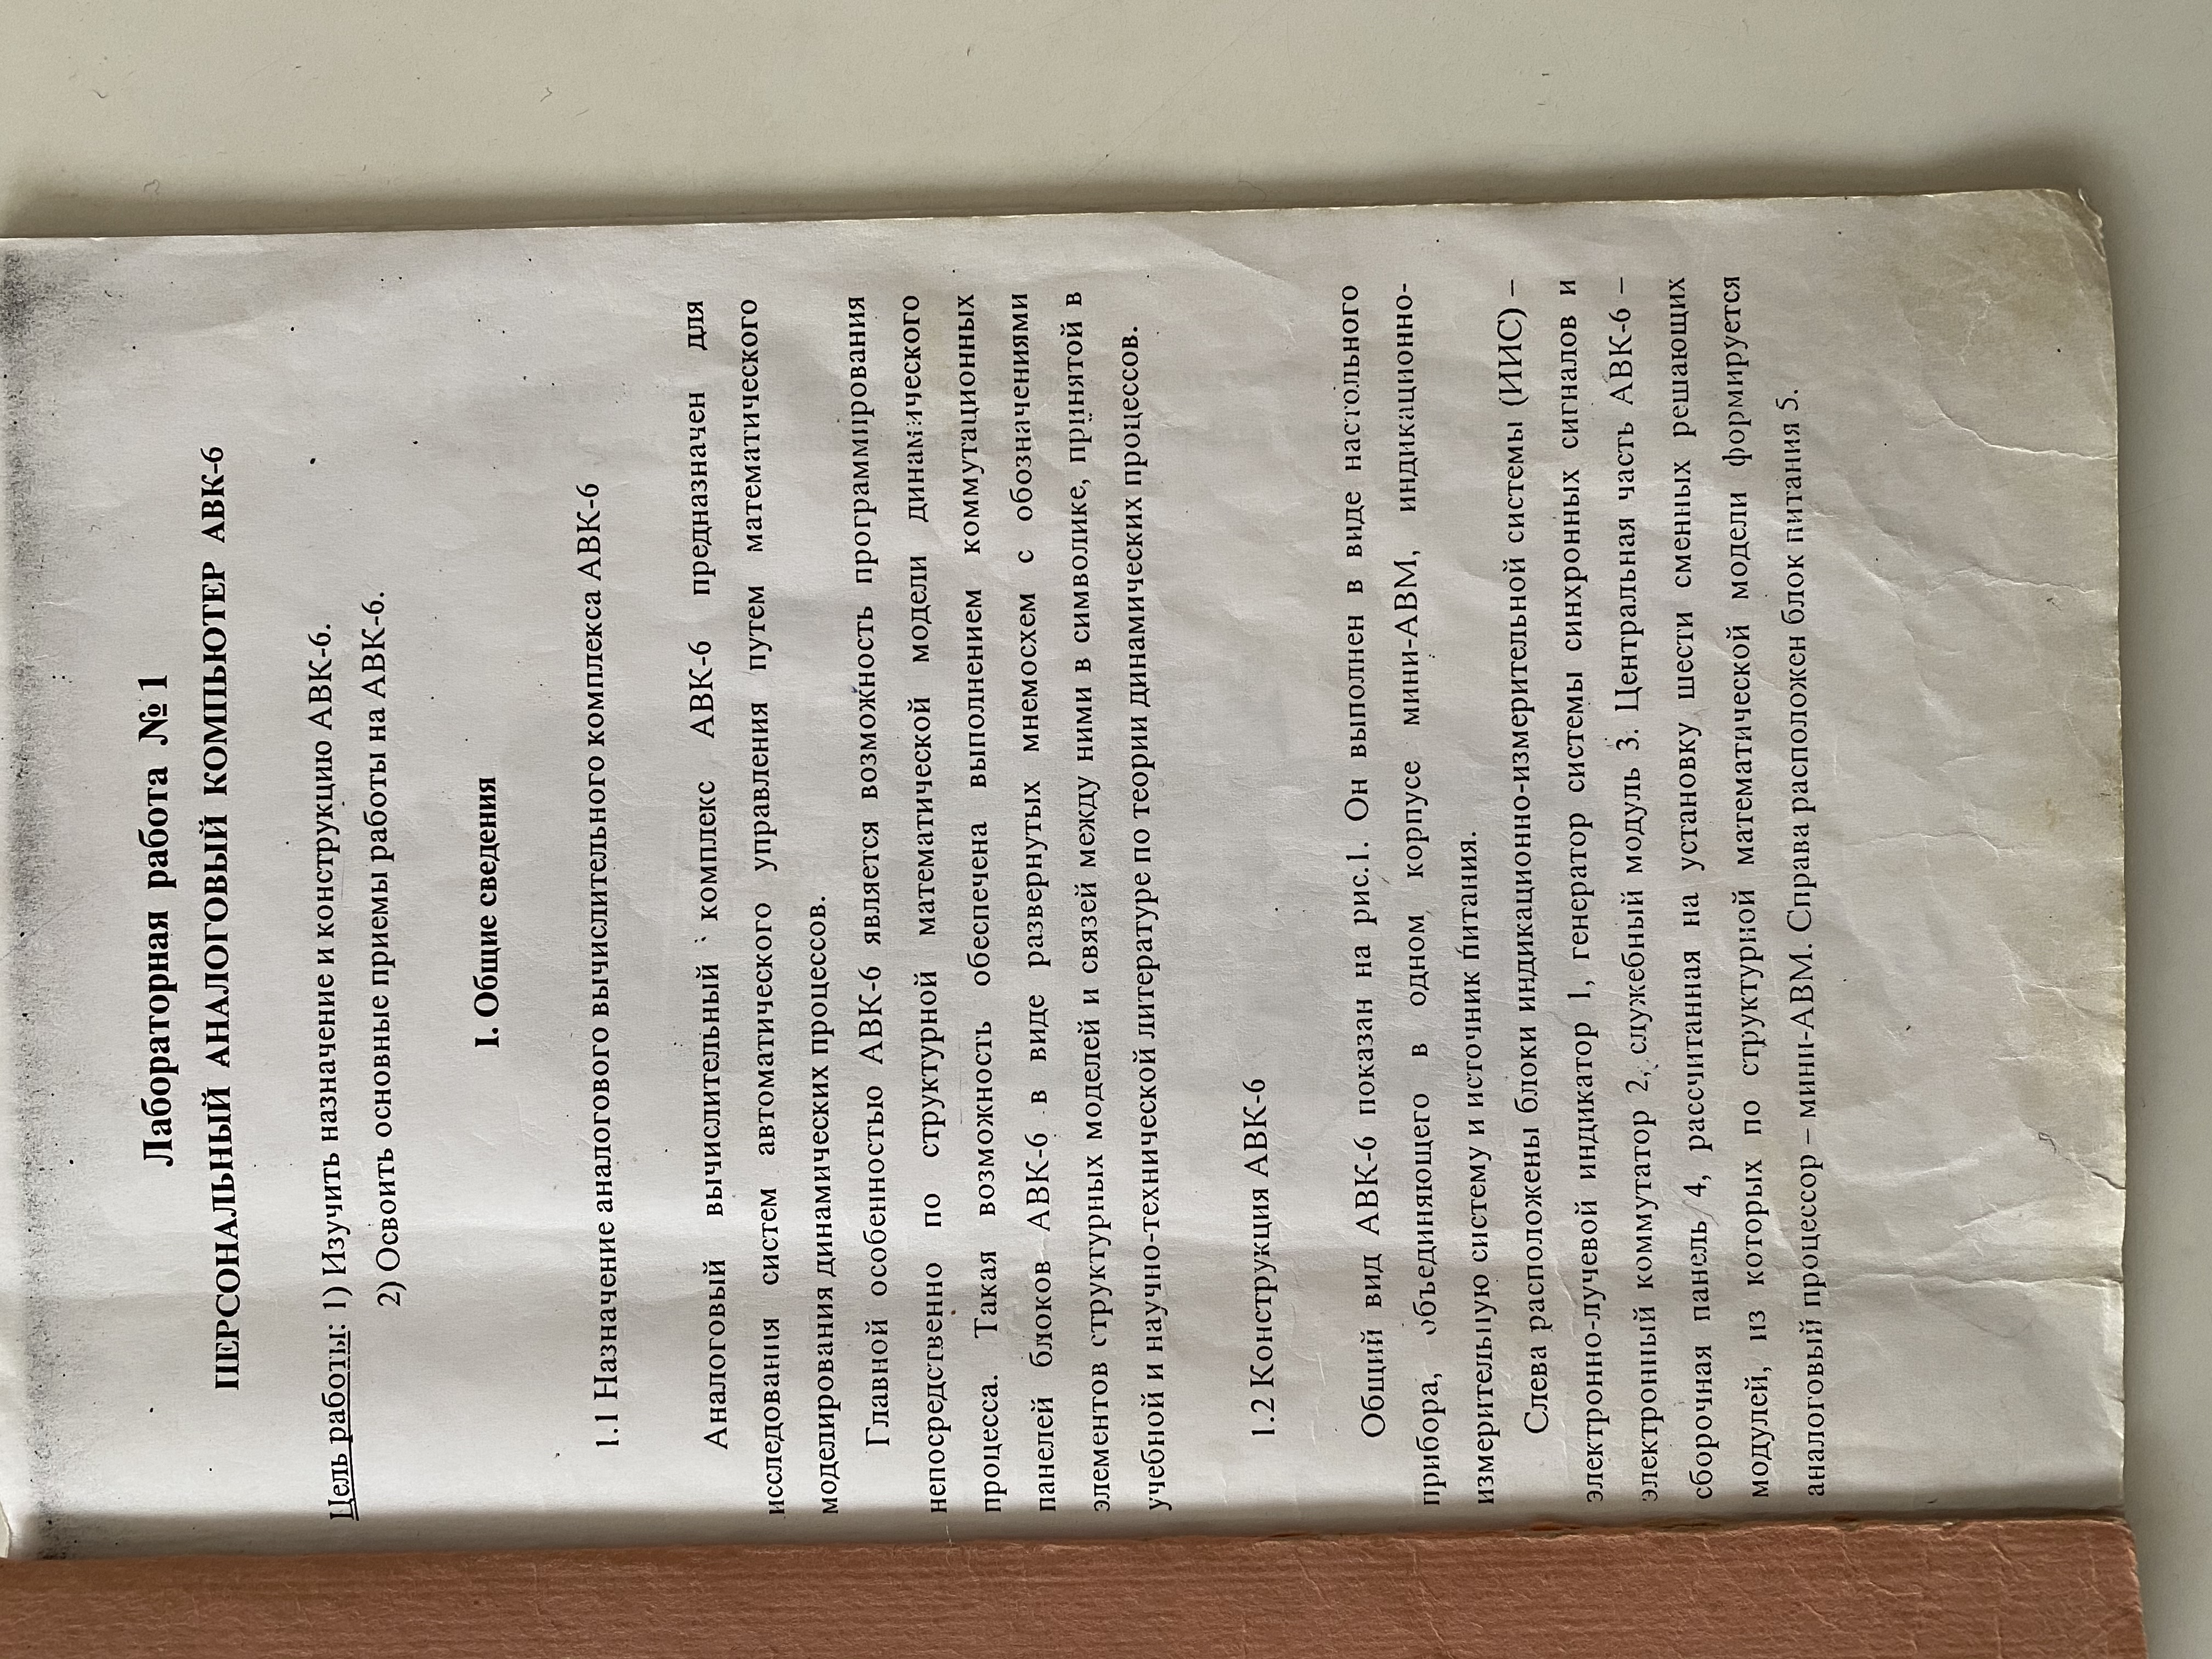
\includegraphics[height = 10 \baselineskip]{./assets/p01.png}
        \caption{Результат виконання розробленої програми}
        \label{fig:app-res}
      \end{figure}

      Як~видно, програма коректно обчислює значення заданого виразу з~вхідними значеннями, заданими у~програмі.

  \section{Висновок}
    Виконуючи дану лабораторну роботу, ми~розробили програму для~заданої паралельної комп'ютерної системи зі~спільною пам'яттю, ознайомились із~процесом розробки паралельних алгоритмів, а~також із~семафорами у~мові програмування «Ада». 

  \appendix
  \section{Програма для~розв'язку поставленої задачі}

    \inputada{../01-solution/lab01.adb}{Початковий код~програмного модуля для~розв'язання задачі}{lst:source-code}

\end{document}
